\documentclass[tikz,border=8pt]{standalone}
% Shared look for every TikZ diagram. Load with \input{../../tools/tikz-style.tex}
\usepackage[T1]{fontenc}
\usepackage{lmodern}
\renewcommand{\sfdefault}{lmr}  % diagrams use the same serif as the text
\usetikzlibrary{arrows.meta, positioning, shapes.geometric, calc, fit, backgrounds}
\definecolor{cblue}{HTML}{4C78A8}
\definecolor{corange}{HTML}{F58518}
\definecolor{cgreen}{HTML}{54A24B}
\definecolor{cred}{HTML}{E45756}
\definecolor{cpurple}{HTML}{B279A2}
\definecolor{cgrey}{HTML}{6B6B6B}
\tikzset{
  every picture/.style={font=\sffamily, line width=1.2pt},
  box/.style={draw=#1, fill=#1!12, rounded corners=4pt, align=center, inner sep=7pt, minimum height=1.1cm},
  box/.default=cgrey,
  arrow/.style={-{Stealth[length=3mm]}, draw=cgrey, line width=1.4pt},
  title/.style={font=\sffamily\bfseries\Large},
  note/.style={font=\sffamily\small, text=cgrey, align=center},
}
\AtBeginDocument{\hyphenpenalty=10000 \exhyphenpenalty=10000}

% Top view of a differential-drive robot: two driven wheels of radius r, separation L, caster, body frame at the axle midpoint.
\begin{document}
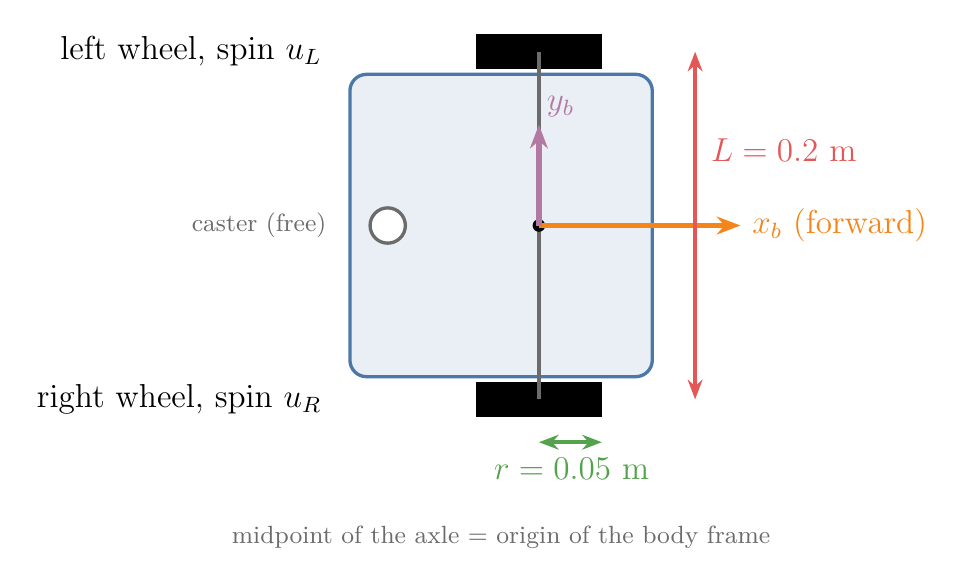
\begin{tikzpicture}[scale=3.2, every node/.append style={font=\large}]
  \draw[cblue, fill=cblue!12, rounded corners=6pt] (-0.75,-0.6) rectangle (0.45,0.6);
  % wheels (seen from above: rectangles of length 2r)
  \fill[black] (-0.25,0.62) rectangle (0.25,0.76);
  \fill[black] (-0.25,-0.76) rectangle (0.25,-0.62);
  \node[anchor=east] at (-0.82,0.69) {left wheel, spin $u_L$};
  \node[anchor=east] at (-0.82,-0.69) {right wheel, spin $u_R$};
  \draw[cgrey, line width=1.6pt] (0,0.69) -- (0,-0.69);
  % caster
  \draw[cgrey, fill=white] (-0.6,0) circle (0.07);
  \node[note, anchor=east] at (-0.8,0) {caster (free)};
  % body frame
  \fill[black] (0,0) circle (0.025);
  \draw[-{Stealth[length=3mm]}, corange, line width=2pt] (0,0) -- (0.8,0) node[right] {$x_b$ (forward)};
  \draw[-{Stealth[length=3mm]}, cpurple, line width=2pt] (0,0) -- (0,0.4) node[above right=-2pt] {$y_b$};
  % L dimension
  \draw[{Stealth[length=2.5mm]}-{Stealth[length=2.5mm]}, cred, line width=1.4pt] (0.62,0.69) -- (0.62,-0.69);
  \node[cred, right] at (0.64,0.3) {$L = 0.2$ m};
  % r dimension
  \draw[{Stealth[length=2.5mm]}-{Stealth[length=2.5mm]}, cgreen, line width=1.4pt] (0,-0.86) -- (0.25,-0.86);
  \node[cgreen, below] at (0.13,-0.88) {$r = 0.05$ m};
  \node[note, anchor=north] at (-0.15,-1.15) {midpoint of the axle = origin of the body frame};
\end{tikzpicture}
\end{document}
